\documentclass[twoside]{book}

% Packages required by doxygen
\usepackage{fixltx2e}
\usepackage{calc}
\usepackage{doxygen}
\usepackage{graphicx}
\usepackage[utf8]{inputenc}
\usepackage{makeidx}
\usepackage{multicol}
\usepackage{multirow}
\PassOptionsToPackage{warn}{textcomp}
\usepackage{textcomp}
\usepackage[nointegrals]{wasysym}
\usepackage[table]{xcolor}

% Font selection
\usepackage[T1]{fontenc}
\usepackage{mathptmx}
\usepackage[scaled=.90]{helvet}
\usepackage{courier}
\usepackage{amssymb}
\usepackage{sectsty}
\renewcommand{\familydefault}{\sfdefault}
\allsectionsfont{%
  \fontseries{bc}\selectfont%
  \color{darkgray}%
}
\renewcommand{\DoxyLabelFont}{%
  \fontseries{bc}\selectfont%
  \color{darkgray}%
}
\newcommand{\+}{\discretionary{\mbox{\scriptsize$\hookleftarrow$}}{}{}}

% Page & text layout
\usepackage{geometry}
\geometry{%
  a4paper,%
  top=2.5cm,%
  bottom=2.5cm,%
  left=2.5cm,%
  right=2.5cm%
}
\tolerance=750
\hfuzz=15pt
\hbadness=750
\setlength{\emergencystretch}{15pt}
\setlength{\parindent}{0cm}
\setlength{\parskip}{0.2cm}
\makeatletter
\renewcommand{\paragraph}{%
  \@startsection{paragraph}{4}{0ex}{-1.0ex}{1.0ex}{%
    \normalfont\normalsize\bfseries\SS@parafont%
  }%
}
\renewcommand{\subparagraph}{%
  \@startsection{subparagraph}{5}{0ex}{-1.0ex}{1.0ex}{%
    \normalfont\normalsize\bfseries\SS@subparafont%
  }%
}
\makeatother

% Headers & footers
\usepackage{fancyhdr}
\pagestyle{fancyplain}
\fancyhead[LE]{\fancyplain{}{\bfseries\thepage}}
\fancyhead[CE]{\fancyplain{}{}}
\fancyhead[RE]{\fancyplain{}{\bfseries\leftmark}}
\fancyhead[LO]{\fancyplain{}{\bfseries\rightmark}}
\fancyhead[CO]{\fancyplain{}{}}
\fancyhead[RO]{\fancyplain{}{\bfseries\thepage}}
\fancyfoot[LE]{\fancyplain{}{}}
\fancyfoot[CE]{\fancyplain{}{}}
\fancyfoot[RE]{\fancyplain{}{\bfseries\scriptsize Generated on Thu Dec 25 2014 16\+:24\+:30 for My Project by Doxygen }}
\fancyfoot[LO]{\fancyplain{}{\bfseries\scriptsize Generated on Thu Dec 25 2014 16\+:24\+:30 for My Project by Doxygen }}
\fancyfoot[CO]{\fancyplain{}{}}
\fancyfoot[RO]{\fancyplain{}{}}
\renewcommand{\footrulewidth}{0.4pt}
\renewcommand{\chaptermark}[1]{%
  \markboth{#1}{}%
}
\renewcommand{\sectionmark}[1]{%
  \markright{\thesection\ #1}%
}

% Indices & bibliography
\usepackage{natbib}
\usepackage[titles]{tocloft}
\setcounter{tocdepth}{3}
\setcounter{secnumdepth}{5}
\makeindex

% Hyperlinks (required, but should be loaded last)
\usepackage{ifpdf}
\ifpdf
  \usepackage[pdftex,pagebackref=true]{hyperref}
\else
  \usepackage[ps2pdf,pagebackref=true]{hyperref}
\fi
\hypersetup{%
  colorlinks=true,%
  linkcolor=blue,%
  citecolor=blue,%
  unicode%
}

% Custom commands
\newcommand{\clearemptydoublepage}{%
  \newpage{\pagestyle{empty}\cleardoublepage}%
}


%===== C O N T E N T S =====

\begin{document}

% Titlepage & ToC
\hypersetup{pageanchor=false,
             bookmarks=true,
             bookmarksnumbered=true,
             pdfencoding=unicode
            }
\pagenumbering{roman}
\begin{titlepage}
\vspace*{7cm}
\begin{center}%
{\Large My Project }\\
\vspace*{1cm}
{\large Generated by Doxygen 1.8.8}\\
\vspace*{0.5cm}
{\small Thu Dec 25 2014 16:24:30}\\
\end{center}
\end{titlepage}
\clearemptydoublepage
\tableofcontents
\clearemptydoublepage
\pagenumbering{arabic}
\hypersetup{pageanchor=true}

%--- Begin generated contents ---
\chapter{Namespace Index}
\section{Namespace List}
Here is a list of all namespaces with brief descriptions\+:\begin{DoxyCompactList}
\item\contentsline{section}{\hyperlink{namespacecategories}{categories} }{\pageref{namespacecategories}}{}
\item\contentsline{section}{\hyperlink{namespace_py_inversion}{Py\+Inversion} }{\pageref{namespace_py_inversion}}{}
\item\contentsline{section}{\hyperlink{namespacezrpc2}{zrpc2} }{\pageref{namespacezrpc2}}{}
\item\contentsline{section}{\hyperlink{namespacezrpcclient}{zrpcclient} }{\pageref{namespacezrpcclient}}{}
\item\contentsline{section}{\hyperlink{namespacezrpcserver}{zrpcserver} }{\pageref{namespacezrpcserver}}{}
\end{DoxyCompactList}

\chapter{Hierarchical Index}
\section{Class Hierarchy}
This inheritance list is sorted roughly, but not completely, alphabetically\+:\begin{DoxyCompactList}
\item \contentsline{section}{Py\+Inversion.\+Feature\+Broker}{\pageref{class_py_inversion_1_1_feature_broker}}{}
\item object\begin{DoxyCompactList}
\item \contentsline{section}{Py\+Inversion.\+Component}{\pageref{class_py_inversion_1_1_component}}{}
\begin{DoxyCompactList}
\item \contentsline{section}{Py\+Inversion.\+Bar}{\pageref{class_py_inversion_1_1_bar}}{}
\item \contentsline{section}{Py\+Inversion.\+Better\+Console}{\pageref{class_py_inversion_1_1_better_console}}{}
\item \contentsline{section}{Py\+Inversion.\+Simple\+Console}{\pageref{class_py_inversion_1_1_simple_console}}{}
\end{DoxyCompactList}
\item \contentsline{section}{Py\+Inversion.\+Required\+Feature}{\pageref{class_py_inversion_1_1_required_feature}}{}
\item \contentsline{section}{zrpcserver.\+Hello\+R\+P\+C}{\pageref{classzrpcserver_1_1_hello_r_p_c}}{}
\end{DoxyCompactList}
\end{DoxyCompactList}

\chapter{Class Index}
\section{Class List}
Here are the classes, structs, unions and interfaces with brief descriptions\+:\begin{DoxyCompactList}
\item\contentsline{section}{\hyperlink{class_py_inversion_1_1_bar}{Py\+Inversion.\+Bar} \\*D\+E\+M\+O }{\pageref{class_py_inversion_1_1_bar}}{}
\item\contentsline{section}{\hyperlink{class_py_inversion_1_1_better_console}{Py\+Inversion.\+Better\+Console} }{\pageref{class_py_inversion_1_1_better_console}}{}
\item\contentsline{section}{\hyperlink{class_py_inversion_1_1_component}{Py\+Inversion.\+Component} }{\pageref{class_py_inversion_1_1_component}}{}
\item\contentsline{section}{\hyperlink{class_py_inversion_1_1_feature_broker}{Py\+Inversion.\+Feature\+Broker} \\*Feature Broker }{\pageref{class_py_inversion_1_1_feature_broker}}{}
\item\contentsline{section}{\hyperlink{classzrpcserver_1_1_hello_r_p_c}{zrpcserver.\+Hello\+R\+P\+C} }{\pageref{classzrpcserver_1_1_hello_r_p_c}}{}
\item\contentsline{section}{\hyperlink{class_py_inversion_1_1_required_feature}{Py\+Inversion.\+Required\+Feature} }{\pageref{class_py_inversion_1_1_required_feature}}{}
\item\contentsline{section}{\hyperlink{class_py_inversion_1_1_simple_console}{Py\+Inversion.\+Simple\+Console} }{\pageref{class_py_inversion_1_1_simple_console}}{}
\end{DoxyCompactList}

\chapter{File Index}
\section{File List}
Here is a list of all files with brief descriptions\+:\begin{DoxyCompactList}
\item\contentsline{section}{D\+:/\+Dropbox/\+A\+S\+C\+O\+N\+Projects/\+Py\+Patterns/\hyperlink{categories_8py}{categories.\+py} }{\pageref{categories_8py}}{}
\item\contentsline{section}{D\+:/\+Dropbox/\+A\+S\+C\+O\+N\+Projects/\+Py\+Patterns/\hyperlink{_py_inversion_8py}{Py\+Inversion.\+py} }{\pageref{_py_inversion_8py}}{}
\item\contentsline{section}{D\+:/\+Dropbox/\+A\+S\+C\+O\+N\+Projects/\+Py\+Patterns/\hyperlink{zrpc2_8py}{zrpc2.\+py} }{\pageref{zrpc2_8py}}{}
\item\contentsline{section}{D\+:/\+Dropbox/\+A\+S\+C\+O\+N\+Projects/\+Py\+Patterns/\hyperlink{zrpcclient_8py}{zrpcclient.\+py} }{\pageref{zrpcclient_8py}}{}
\item\contentsline{section}{D\+:/\+Dropbox/\+A\+S\+C\+O\+N\+Projects/\+Py\+Patterns/\hyperlink{zrpcserver_8py}{zrpcserver.\+py} }{\pageref{zrpcserver_8py}}{}
\end{DoxyCompactList}

\chapter{Namespace Documentation}
\hypertarget{namespacecategories}{\section{categories Namespace Reference}
\label{namespacecategories}\index{categories@{categories}}
}
\subsection*{Functions}
\begin{DoxyCompactItemize}
\item 
def \hyperlink{namespacecategories_ad5d3141fa655736c1fccef95069bf138}{identity}
\item 
def \hyperlink{namespacecategories_a8c3eb907e91bca8102418150ca6db3fd}{plusone}
\item 
def \hyperlink{namespacecategories_a4e763f6d2815828e12fcfea9bc54ddb8}{comp}
\end{DoxyCompactItemize}
\subsection*{Variables}
\begin{DoxyCompactItemize}
\item 
tuple \hyperlink{namespacecategories_aa6ad1b25eda2dc4703279de8c42636c3}{a} = \hyperlink{namespacecategories_ad5d3141fa655736c1fccef95069bf138}{identity}(\char`\"{}11\char`\"{})
\end{DoxyCompactItemize}


\subsection{Function Documentation}
\hypertarget{namespacecategories_a4e763f6d2815828e12fcfea9bc54ddb8}{\index{categories@{categories}!comp@{comp}}
\index{comp@{comp}!categories@{categories}}
\subsubsection[{comp}]{\setlength{\rightskip}{0pt plus 5cm}def categories.\+comp (
\begin{DoxyParamCaption}
\item[{}]{f1, }
\item[{}]{f2}
\end{DoxyParamCaption}
)}}\label{namespacecategories_a4e763f6d2815828e12fcfea9bc54ddb8}
\begin{DoxyVerb}:type f1: function
:type f2: function
:rtype: function
\end{DoxyVerb}
 \hypertarget{namespacecategories_ad5d3141fa655736c1fccef95069bf138}{\index{categories@{categories}!identity@{identity}}
\index{identity@{identity}!categories@{categories}}
\subsubsection[{identity}]{\setlength{\rightskip}{0pt plus 5cm}def categories.\+identity (
\begin{DoxyParamCaption}
\item[{}]{x}
\end{DoxyParamCaption}
)}}\label{namespacecategories_ad5d3141fa655736c1fccef95069bf138}
\begin{DoxyVerb}:type f1: object
:type f2: object
:rtype: object
\end{DoxyVerb}
 \hypertarget{namespacecategories_a8c3eb907e91bca8102418150ca6db3fd}{\index{categories@{categories}!plusone@{plusone}}
\index{plusone@{plusone}!categories@{categories}}
\subsubsection[{plusone}]{\setlength{\rightskip}{0pt plus 5cm}def categories.\+plusone (
\begin{DoxyParamCaption}
\item[{}]{x}
\end{DoxyParamCaption}
)}}\label{namespacecategories_a8c3eb907e91bca8102418150ca6db3fd}


\subsection{Variable Documentation}
\hypertarget{namespacecategories_aa6ad1b25eda2dc4703279de8c42636c3}{\index{categories@{categories}!a@{a}}
\index{a@{a}!categories@{categories}}
\subsubsection[{a}]{\setlength{\rightskip}{0pt plus 5cm}tuple categories.\+a = {\bf identity}(\char`\"{}11\char`\"{})}}\label{namespacecategories_aa6ad1b25eda2dc4703279de8c42636c3}

\hypertarget{namespace_py_inversion}{\section{Py\+Inversion Namespace Reference}
\label{namespace_py_inversion}\index{Py\+Inversion@{Py\+Inversion}}
}
\subsection*{Classes}
\begin{DoxyCompactItemize}
\item 
class \hyperlink{class_py_inversion_1_1_bar}{Bar}
\begin{DoxyCompactList}\small\item\em D\+E\+M\+O. \end{DoxyCompactList}\item 
class \hyperlink{class_py_inversion_1_1_better_console}{Better\+Console}
\item 
class \hyperlink{class_py_inversion_1_1_component}{Component}
\item 
class \hyperlink{class_py_inversion_1_1_feature_broker}{Feature\+Broker}
\begin{DoxyCompactList}\small\item\em Feature Broker. \end{DoxyCompactList}\item 
class \hyperlink{class_py_inversion_1_1_required_feature}{Required\+Feature}
\item 
class \hyperlink{class_py_inversion_1_1_simple_console}{Simple\+Console}
\end{DoxyCompactItemize}
\subsection*{Functions}
\begin{DoxyCompactItemize}
\item 
def \hyperlink{namespace_py_inversion_a188b1a2e50ba7079abd28f76308d8ee1}{No\+Assertion}
\begin{DoxyCompactList}\small\item\em Representation of Required Features and Feature Assertions. \end{DoxyCompactList}\item 
def \hyperlink{namespace_py_inversion_aef868798a7eac8ca225dd912b28ee196}{Is\+Instance\+Of}
\item 
def \hyperlink{namespace_py_inversion_ae61281915fdeaebe010d9660152ed2b5}{Has\+Attributes}
\item 
def \hyperlink{namespace_py_inversion_aa26f41ad968118f6feb4f754492b9246}{Has\+Methods}
\item 
def \hyperlink{namespace_py_inversion_aa73efe236b02a8a53f625fd15ec22ef2}{Get\+Current\+User}
\end{DoxyCompactItemize}
\subsection*{Variables}
\begin{DoxyCompactItemize}
\item 
string \hyperlink{namespace_py_inversion_a75d60c831488f0073dfa93077eeb6645}{\+\_\+\+\_\+author\+\_\+\+\_\+} = 'bausk'
\item 
tuple \hyperlink{namespace_py_inversion_a83916a9bd83dabb820f9756e0d6e9bc5}{features} = \hyperlink{class_py_inversion_1_1_feature_broker}{Feature\+Broker}()
\item 
tuple \hyperlink{namespace_py_inversion_a2744d30b0d1932d2fc87d21291bb5a1a}{bar} = \hyperlink{class_py_inversion_1_1_bar}{Bar}()
\begin{DoxyCompactList}\small\item\em features.\+Provide('Console', \hyperlink{class_py_inversion_1_1_better_console}{Better\+Console}(prefix='--$>$')) \# $<$-- singleton lifestyle \end{DoxyCompactList}\end{DoxyCompactItemize}


\subsection{Function Documentation}
\hypertarget{namespace_py_inversion_aa73efe236b02a8a53f625fd15ec22ef2}{\index{Py\+Inversion@{Py\+Inversion}!Get\+Current\+User@{Get\+Current\+User}}
\index{Get\+Current\+User@{Get\+Current\+User}!Py\+Inversion@{Py\+Inversion}}
\subsubsection[{Get\+Current\+User}]{\setlength{\rightskip}{0pt plus 5cm}def Py\+Inversion.\+Get\+Current\+User (
\begin{DoxyParamCaption}
{}
\end{DoxyParamCaption}
)}}\label{namespace_py_inversion_aa73efe236b02a8a53f625fd15ec22ef2}
\hypertarget{namespace_py_inversion_ae61281915fdeaebe010d9660152ed2b5}{\index{Py\+Inversion@{Py\+Inversion}!Has\+Attributes@{Has\+Attributes}}
\index{Has\+Attributes@{Has\+Attributes}!Py\+Inversion@{Py\+Inversion}}
\subsubsection[{Has\+Attributes}]{\setlength{\rightskip}{0pt plus 5cm}def Py\+Inversion.\+Has\+Attributes (
\begin{DoxyParamCaption}
\item[{}]{attributes}
\end{DoxyParamCaption}
)}}\label{namespace_py_inversion_ae61281915fdeaebe010d9660152ed2b5}
\hypertarget{namespace_py_inversion_aa26f41ad968118f6feb4f754492b9246}{\index{Py\+Inversion@{Py\+Inversion}!Has\+Methods@{Has\+Methods}}
\index{Has\+Methods@{Has\+Methods}!Py\+Inversion@{Py\+Inversion}}
\subsubsection[{Has\+Methods}]{\setlength{\rightskip}{0pt plus 5cm}def Py\+Inversion.\+Has\+Methods (
\begin{DoxyParamCaption}
\item[{}]{methods}
\end{DoxyParamCaption}
)}}\label{namespace_py_inversion_aa26f41ad968118f6feb4f754492b9246}
\hypertarget{namespace_py_inversion_aef868798a7eac8ca225dd912b28ee196}{\index{Py\+Inversion@{Py\+Inversion}!Is\+Instance\+Of@{Is\+Instance\+Of}}
\index{Is\+Instance\+Of@{Is\+Instance\+Of}!Py\+Inversion@{Py\+Inversion}}
\subsubsection[{Is\+Instance\+Of}]{\setlength{\rightskip}{0pt plus 5cm}def Py\+Inversion.\+Is\+Instance\+Of (
\begin{DoxyParamCaption}
\item[{}]{classes}
\end{DoxyParamCaption}
)}}\label{namespace_py_inversion_aef868798a7eac8ca225dd912b28ee196}
\hypertarget{namespace_py_inversion_a188b1a2e50ba7079abd28f76308d8ee1}{\index{Py\+Inversion@{Py\+Inversion}!No\+Assertion@{No\+Assertion}}
\index{No\+Assertion@{No\+Assertion}!Py\+Inversion@{Py\+Inversion}}
\subsubsection[{No\+Assertion}]{\setlength{\rightskip}{0pt plus 5cm}def Py\+Inversion.\+No\+Assertion (
\begin{DoxyParamCaption}
\item[{}]{obj}
\end{DoxyParamCaption}
)}}\label{namespace_py_inversion_a188b1a2e50ba7079abd28f76308d8ee1}


Representation of Required Features and Feature Assertions. 



\subsection{Variable Documentation}
\hypertarget{namespace_py_inversion_a75d60c831488f0073dfa93077eeb6645}{\index{Py\+Inversion@{Py\+Inversion}!\+\_\+\+\_\+author\+\_\+\+\_\+@{\+\_\+\+\_\+author\+\_\+\+\_\+}}
\index{\+\_\+\+\_\+author\+\_\+\+\_\+@{\+\_\+\+\_\+author\+\_\+\+\_\+}!Py\+Inversion@{Py\+Inversion}}
\subsubsection[{\+\_\+\+\_\+author\+\_\+\+\_\+}]{\setlength{\rightskip}{0pt plus 5cm}string Py\+Inversion.\+\_\+\+\_\+author\+\_\+\+\_\+ = 'bausk'}}\label{namespace_py_inversion_a75d60c831488f0073dfa93077eeb6645}
\hypertarget{namespace_py_inversion_a2744d30b0d1932d2fc87d21291bb5a1a}{\index{Py\+Inversion@{Py\+Inversion}!bar@{bar}}
\index{bar@{bar}!Py\+Inversion@{Py\+Inversion}}
\subsubsection[{bar}]{\setlength{\rightskip}{0pt plus 5cm}tuple Py\+Inversion.\+bar = {\bf Bar}()}}\label{namespace_py_inversion_a2744d30b0d1932d2fc87d21291bb5a1a}


features.\+Provide('Console', \hyperlink{class_py_inversion_1_1_better_console}{Better\+Console}(prefix='--$>$')) \# $<$-- singleton lifestyle 

\hypertarget{namespace_py_inversion_a83916a9bd83dabb820f9756e0d6e9bc5}{\index{Py\+Inversion@{Py\+Inversion}!features@{features}}
\index{features@{features}!Py\+Inversion@{Py\+Inversion}}
\subsubsection[{features}]{\setlength{\rightskip}{0pt plus 5cm}tuple Py\+Inversion.\+features = {\bf Feature\+Broker}()}}\label{namespace_py_inversion_a83916a9bd83dabb820f9756e0d6e9bc5}

\hypertarget{namespacezrpc2}{\section{zrpc2 Namespace Reference}
\label{namespacezrpc2}\index{zrpc2@{zrpc2}}
}
\subsection*{Variables}
\begin{DoxyCompactItemize}
\item 
string \hyperlink{namespacezrpc2_ab6eb50c4b8d874520e4089b273b63e16}{\+\_\+\+\_\+author\+\_\+\+\_\+} = 'bausk'
\item 
tuple \hyperlink{namespacezrpc2_aad77b0202c8bdc01b68d63c381d5bb4b}{context} = zmq.\+Context()
\item 
tuple \hyperlink{namespacezrpc2_a5cc44b717d0374316398080bedecec05}{socket} = context.\+socket(zmq.\+R\+E\+P)
\item 
tuple \hyperlink{namespacezrpc2_a3a2870282951b1ba168443ba71d13079}{message} = socket.\+recv()
\item 
tuple \hyperlink{namespacezrpc2_a55892ab0cec9d46ce8b2a50f92998e57}{m2} = msgpack.\+unpackb(\hyperlink{namespacezrpc2_a3a2870282951b1ba168443ba71d13079}{message})
\end{DoxyCompactItemize}


\subsection{Variable Documentation}
\hypertarget{namespacezrpc2_ab6eb50c4b8d874520e4089b273b63e16}{\index{zrpc2@{zrpc2}!\+\_\+\+\_\+author\+\_\+\+\_\+@{\+\_\+\+\_\+author\+\_\+\+\_\+}}
\index{\+\_\+\+\_\+author\+\_\+\+\_\+@{\+\_\+\+\_\+author\+\_\+\+\_\+}!zrpc2@{zrpc2}}
\subsubsection[{\+\_\+\+\_\+author\+\_\+\+\_\+}]{\setlength{\rightskip}{0pt plus 5cm}string zrpc2.\+\_\+\+\_\+author\+\_\+\+\_\+ = 'bausk'}}\label{namespacezrpc2_ab6eb50c4b8d874520e4089b273b63e16}
\hypertarget{namespacezrpc2_aad77b0202c8bdc01b68d63c381d5bb4b}{\index{zrpc2@{zrpc2}!context@{context}}
\index{context@{context}!zrpc2@{zrpc2}}
\subsubsection[{context}]{\setlength{\rightskip}{0pt plus 5cm}tuple zrpc2.\+context = zmq.\+Context()}}\label{namespacezrpc2_aad77b0202c8bdc01b68d63c381d5bb4b}
\hypertarget{namespacezrpc2_a55892ab0cec9d46ce8b2a50f92998e57}{\index{zrpc2@{zrpc2}!m2@{m2}}
\index{m2@{m2}!zrpc2@{zrpc2}}
\subsubsection[{m2}]{\setlength{\rightskip}{0pt plus 5cm}tuple zrpc2.\+m2 = msgpack.\+unpackb({\bf message})}}\label{namespacezrpc2_a55892ab0cec9d46ce8b2a50f92998e57}
\hypertarget{namespacezrpc2_a3a2870282951b1ba168443ba71d13079}{\index{zrpc2@{zrpc2}!message@{message}}
\index{message@{message}!zrpc2@{zrpc2}}
\subsubsection[{message}]{\setlength{\rightskip}{0pt plus 5cm}tuple zrpc2.\+message = socket.\+recv()}}\label{namespacezrpc2_a3a2870282951b1ba168443ba71d13079}
\hypertarget{namespacezrpc2_a5cc44b717d0374316398080bedecec05}{\index{zrpc2@{zrpc2}!socket@{socket}}
\index{socket@{socket}!zrpc2@{zrpc2}}
\subsubsection[{socket}]{\setlength{\rightskip}{0pt plus 5cm}tuple zrpc2.\+socket = context.\+socket(zmq.\+R\+E\+P)}}\label{namespacezrpc2_a5cc44b717d0374316398080bedecec05}

\hypertarget{namespacezrpcclient}{\section{zrpcclient Namespace Reference}
\label{namespacezrpcclient}\index{zrpcclient@{zrpcclient}}
}
\subsection*{Variables}
\begin{DoxyCompactItemize}
\item 
tuple \hyperlink{namespacezrpcclient_a039edf63871343a5809f1e216cc7e5cd}{c} = zerorpc.\+Client()
\end{DoxyCompactItemize}


\subsection{Variable Documentation}
\hypertarget{namespacezrpcclient_a039edf63871343a5809f1e216cc7e5cd}{\index{zrpcclient@{zrpcclient}!c@{c}}
\index{c@{c}!zrpcclient@{zrpcclient}}
\subsubsection[{c}]{\setlength{\rightskip}{0pt plus 5cm}tuple zrpcclient.\+c = zerorpc.\+Client()}}\label{namespacezrpcclient_a039edf63871343a5809f1e216cc7e5cd}

\hypertarget{namespacezrpcserver}{\section{zrpcserver Namespace Reference}
\label{namespacezrpcserver}\index{zrpcserver@{zrpcserver}}
}
\subsection*{Classes}
\begin{DoxyCompactItemize}
\item 
class \hyperlink{classzrpcserver_1_1_hello_r_p_c}{Hello\+R\+P\+C}
\end{DoxyCompactItemize}
\subsection*{Variables}
\begin{DoxyCompactItemize}
\item 
tuple \hyperlink{namespacezrpcserver_a27c4be0435b479044d8544312829e19f}{s} = zerorpc.\+Server(\hyperlink{classzrpcserver_1_1_hello_r_p_c}{Hello\+R\+P\+C}())
\item 
tuple \hyperlink{namespacezrpcserver_aba2558901917b86cf74044e3313df8d8}{context} = zmq.\+Context()
\item 
tuple \hyperlink{namespacezrpcserver_a5e4952d9f1e8548ca60fc87e02414711}{socket} = context.\+socket(zmq.\+R\+E\+P)
\item 
tuple \hyperlink{namespacezrpcserver_a3cf2b2246b68a156037b2a86b71282ff}{message} = socket.\+recv()
\item 
tuple \hyperlink{namespacezrpcserver_a867cc3b9e35ae551991976a86a47829d}{m2} = msgpack.\+unpackb(\hyperlink{namespacezrpcserver_a3cf2b2246b68a156037b2a86b71282ff}{message})
\end{DoxyCompactItemize}


\subsection{Variable Documentation}
\hypertarget{namespacezrpcserver_aba2558901917b86cf74044e3313df8d8}{\index{zrpcserver@{zrpcserver}!context@{context}}
\index{context@{context}!zrpcserver@{zrpcserver}}
\subsubsection[{context}]{\setlength{\rightskip}{0pt plus 5cm}tuple zrpcserver.\+context = zmq.\+Context()}}\label{namespacezrpcserver_aba2558901917b86cf74044e3313df8d8}
\hypertarget{namespacezrpcserver_a867cc3b9e35ae551991976a86a47829d}{\index{zrpcserver@{zrpcserver}!m2@{m2}}
\index{m2@{m2}!zrpcserver@{zrpcserver}}
\subsubsection[{m2}]{\setlength{\rightskip}{0pt plus 5cm}tuple zrpcserver.\+m2 = msgpack.\+unpackb({\bf message})}}\label{namespacezrpcserver_a867cc3b9e35ae551991976a86a47829d}
\hypertarget{namespacezrpcserver_a3cf2b2246b68a156037b2a86b71282ff}{\index{zrpcserver@{zrpcserver}!message@{message}}
\index{message@{message}!zrpcserver@{zrpcserver}}
\subsubsection[{message}]{\setlength{\rightskip}{0pt plus 5cm}tuple zrpcserver.\+message = socket.\+recv()}}\label{namespacezrpcserver_a3cf2b2246b68a156037b2a86b71282ff}
\hypertarget{namespacezrpcserver_a27c4be0435b479044d8544312829e19f}{\index{zrpcserver@{zrpcserver}!s@{s}}
\index{s@{s}!zrpcserver@{zrpcserver}}
\subsubsection[{s}]{\setlength{\rightskip}{0pt plus 5cm}tuple zrpcserver.\+s = zerorpc.\+Server({\bf Hello\+R\+P\+C}())}}\label{namespacezrpcserver_a27c4be0435b479044d8544312829e19f}
\hypertarget{namespacezrpcserver_a5e4952d9f1e8548ca60fc87e02414711}{\index{zrpcserver@{zrpcserver}!socket@{socket}}
\index{socket@{socket}!zrpcserver@{zrpcserver}}
\subsubsection[{socket}]{\setlength{\rightskip}{0pt plus 5cm}tuple zrpcserver.\+socket = context.\+socket(zmq.\+R\+E\+P)}}\label{namespacezrpcserver_a5e4952d9f1e8548ca60fc87e02414711}

\chapter{Class Documentation}
\hypertarget{class_py_inversion_1_1_bar}{\section{Py\+Inversion.\+Bar Class Reference}
\label{class_py_inversion_1_1_bar}\index{Py\+Inversion.\+Bar@{Py\+Inversion.\+Bar}}
}


D\+E\+M\+O.  


Inheritance diagram for Py\+Inversion.\+Bar\+:\begin{figure}[H]
\begin{center}
\leavevmode
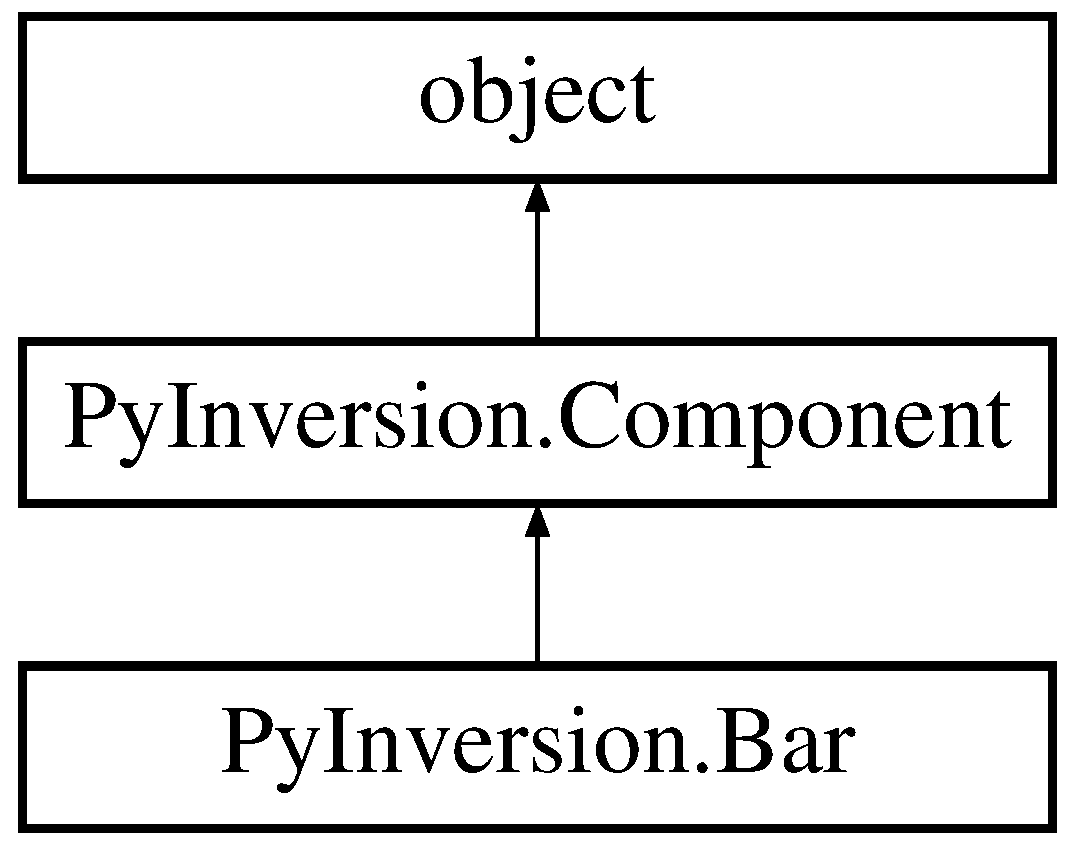
\includegraphics[height=3.000000cm]{class_py_inversion_1_1_bar}
\end{center}
\end{figure}
\subsection*{Public Member Functions}
\begin{DoxyCompactItemize}
\item 
def \hyperlink{class_py_inversion_1_1_bar_a5260b893217bbc99f5a64093a58f3f2e}{\+\_\+\+\_\+init\+\_\+\+\_\+}
\item 
def \hyperlink{class_py_inversion_1_1_bar_a79ffcb7acf21e83f7ce3d60231adef36}{Print\+Yourself}
\end{DoxyCompactItemize}
\subsection*{Public Attributes}
\begin{DoxyCompactItemize}
\item 
\hyperlink{class_py_inversion_1_1_bar_a40572207d252c893b1e9b91005dd21b3}{X}
\end{DoxyCompactItemize}
\subsection*{Static Public Attributes}
\begin{DoxyCompactItemize}
\item 
tuple \hyperlink{class_py_inversion_1_1_bar_a8c5a4e5d2e87d13da13ee91237755c68}{con} = \hyperlink{class_py_inversion_1_1_required_feature}{Required\+Feature}('Console', \hyperlink{namespace_py_inversion_aa26f41ad968118f6feb4f754492b9246}{Has\+Methods}('Write\+Line'))
\item 
tuple \hyperlink{class_py_inversion_1_1_bar_a479c6f234727e5c616429c16dd81ac1f}{title} = \hyperlink{class_py_inversion_1_1_required_feature}{Required\+Feature}('App\+Title', \hyperlink{namespace_py_inversion_aef868798a7eac8ca225dd912b28ee196}{Is\+Instance\+Of}(str))
\item 
tuple \hyperlink{class_py_inversion_1_1_bar_a24c2b32467d45551a2ba8cd20c6749f4}{user} = \hyperlink{class_py_inversion_1_1_required_feature}{Required\+Feature}('Current\+User', \hyperlink{namespace_py_inversion_aef868798a7eac8ca225dd912b28ee196}{Is\+Instance\+Of}(str))
\end{DoxyCompactItemize}


\subsection{Detailed Description}
D\+E\+M\+O. 



\subsection{Constructor \& Destructor Documentation}
\hypertarget{class_py_inversion_1_1_bar_a5260b893217bbc99f5a64093a58f3f2e}{\index{Py\+Inversion\+::\+Bar@{Py\+Inversion\+::\+Bar}!\+\_\+\+\_\+init\+\_\+\+\_\+@{\+\_\+\+\_\+init\+\_\+\+\_\+}}
\index{\+\_\+\+\_\+init\+\_\+\+\_\+@{\+\_\+\+\_\+init\+\_\+\+\_\+}!Py\+Inversion\+::\+Bar@{Py\+Inversion\+::\+Bar}}
\subsubsection[{\+\_\+\+\_\+init\+\_\+\+\_\+}]{\setlength{\rightskip}{0pt plus 5cm}def Py\+Inversion.\+Bar.\+\_\+\+\_\+init\+\_\+\+\_\+ (
\begin{DoxyParamCaption}
\item[{}]{self}
\end{DoxyParamCaption}
)}}\label{class_py_inversion_1_1_bar_a5260b893217bbc99f5a64093a58f3f2e}


\subsection{Member Function Documentation}
\hypertarget{class_py_inversion_1_1_bar_a79ffcb7acf21e83f7ce3d60231adef36}{\index{Py\+Inversion\+::\+Bar@{Py\+Inversion\+::\+Bar}!Print\+Yourself@{Print\+Yourself}}
\index{Print\+Yourself@{Print\+Yourself}!Py\+Inversion\+::\+Bar@{Py\+Inversion\+::\+Bar}}
\subsubsection[{Print\+Yourself}]{\setlength{\rightskip}{0pt plus 5cm}def Py\+Inversion.\+Bar.\+Print\+Yourself (
\begin{DoxyParamCaption}
\item[{}]{self}
\end{DoxyParamCaption}
)}}\label{class_py_inversion_1_1_bar_a79ffcb7acf21e83f7ce3d60231adef36}


\subsection{Member Data Documentation}
\hypertarget{class_py_inversion_1_1_bar_a8c5a4e5d2e87d13da13ee91237755c68}{\index{Py\+Inversion\+::\+Bar@{Py\+Inversion\+::\+Bar}!con@{con}}
\index{con@{con}!Py\+Inversion\+::\+Bar@{Py\+Inversion\+::\+Bar}}
\subsubsection[{con}]{\setlength{\rightskip}{0pt plus 5cm}tuple Py\+Inversion.\+Bar.\+con = {\bf Required\+Feature}('Console', {\bf Has\+Methods}('Write\+Line'))\hspace{0.3cm}{\ttfamily [static]}}}\label{class_py_inversion_1_1_bar_a8c5a4e5d2e87d13da13ee91237755c68}
\hypertarget{class_py_inversion_1_1_bar_a479c6f234727e5c616429c16dd81ac1f}{\index{Py\+Inversion\+::\+Bar@{Py\+Inversion\+::\+Bar}!title@{title}}
\index{title@{title}!Py\+Inversion\+::\+Bar@{Py\+Inversion\+::\+Bar}}
\subsubsection[{title}]{\setlength{\rightskip}{0pt plus 5cm}tuple Py\+Inversion.\+Bar.\+title = {\bf Required\+Feature}('App\+Title', {\bf Is\+Instance\+Of}(str))\hspace{0.3cm}{\ttfamily [static]}}}\label{class_py_inversion_1_1_bar_a479c6f234727e5c616429c16dd81ac1f}
\hypertarget{class_py_inversion_1_1_bar_a24c2b32467d45551a2ba8cd20c6749f4}{\index{Py\+Inversion\+::\+Bar@{Py\+Inversion\+::\+Bar}!user@{user}}
\index{user@{user}!Py\+Inversion\+::\+Bar@{Py\+Inversion\+::\+Bar}}
\subsubsection[{user}]{\setlength{\rightskip}{0pt plus 5cm}tuple Py\+Inversion.\+Bar.\+user = {\bf Required\+Feature}('Current\+User', {\bf Is\+Instance\+Of}(str))\hspace{0.3cm}{\ttfamily [static]}}}\label{class_py_inversion_1_1_bar_a24c2b32467d45551a2ba8cd20c6749f4}
\hypertarget{class_py_inversion_1_1_bar_a40572207d252c893b1e9b91005dd21b3}{\index{Py\+Inversion\+::\+Bar@{Py\+Inversion\+::\+Bar}!X@{X}}
\index{X@{X}!Py\+Inversion\+::\+Bar@{Py\+Inversion\+::\+Bar}}
\subsubsection[{X}]{\setlength{\rightskip}{0pt plus 5cm}Py\+Inversion.\+Bar.\+X}}\label{class_py_inversion_1_1_bar_a40572207d252c893b1e9b91005dd21b3}


The documentation for this class was generated from the following file\+:\begin{DoxyCompactItemize}
\item 
D\+:/\+Dropbox/\+A\+S\+C\+O\+N\+Projects/\+Py\+Patterns/\hyperlink{_py_inversion_8py}{Py\+Inversion.\+py}\end{DoxyCompactItemize}

\hypertarget{class_py_inversion_1_1_better_console}{\section{Py\+Inversion.\+Better\+Console Class Reference}
\label{class_py_inversion_1_1_better_console}\index{Py\+Inversion.\+Better\+Console@{Py\+Inversion.\+Better\+Console}}
}
Inheritance diagram for Py\+Inversion.\+Better\+Console\+:\begin{figure}[H]
\begin{center}
\leavevmode
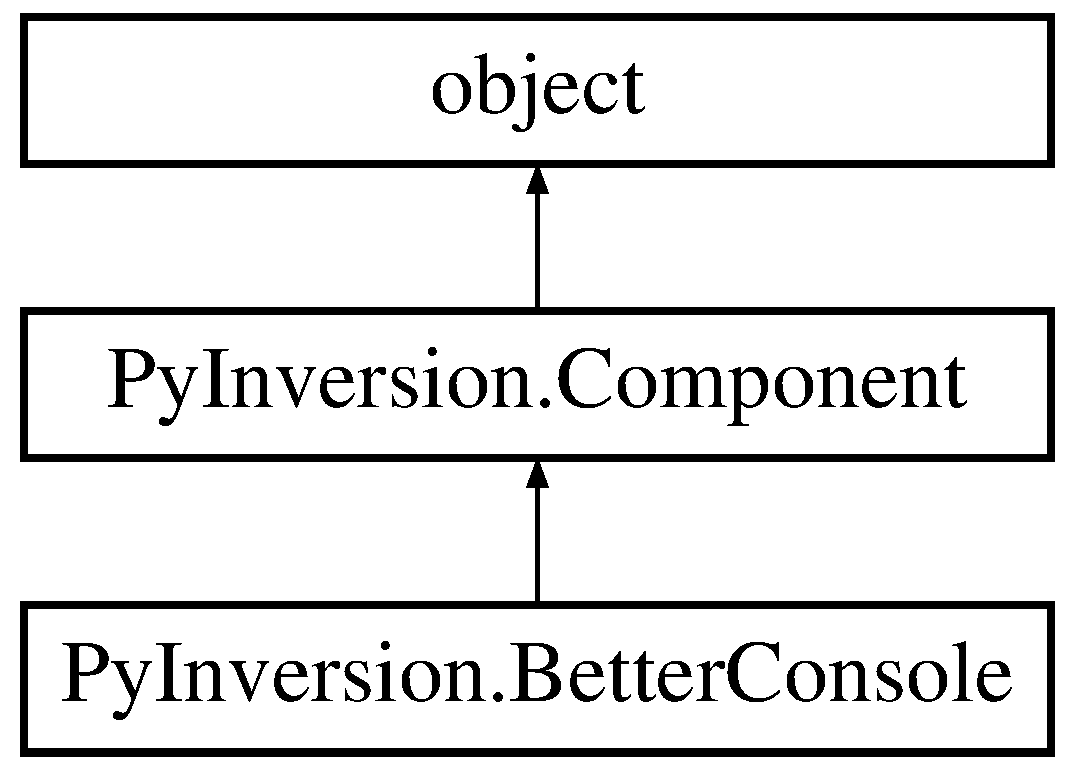
\includegraphics[height=3.000000cm]{class_py_inversion_1_1_better_console}
\end{center}
\end{figure}
\subsection*{Public Member Functions}
\begin{DoxyCompactItemize}
\item 
def \hyperlink{class_py_inversion_1_1_better_console_a27d4e7297fede33e118f2fcea85261d7}{\+\_\+\+\_\+init\+\_\+\+\_\+}
\item 
def \hyperlink{class_py_inversion_1_1_better_console_a7ecf3b24bfa992fc4efed64bed01c2dd}{Write\+Line}
\end{DoxyCompactItemize}
\subsection*{Public Attributes}
\begin{DoxyCompactItemize}
\item 
\hyperlink{class_py_inversion_1_1_better_console_a8346f680b0eb800069f30982947895d2}{prefix}
\end{DoxyCompactItemize}


\subsection{Constructor \& Destructor Documentation}
\hypertarget{class_py_inversion_1_1_better_console_a27d4e7297fede33e118f2fcea85261d7}{\index{Py\+Inversion\+::\+Better\+Console@{Py\+Inversion\+::\+Better\+Console}!\+\_\+\+\_\+init\+\_\+\+\_\+@{\+\_\+\+\_\+init\+\_\+\+\_\+}}
\index{\+\_\+\+\_\+init\+\_\+\+\_\+@{\+\_\+\+\_\+init\+\_\+\+\_\+}!Py\+Inversion\+::\+Better\+Console@{Py\+Inversion\+::\+Better\+Console}}
\subsubsection[{\+\_\+\+\_\+init\+\_\+\+\_\+}]{\setlength{\rightskip}{0pt plus 5cm}def Py\+Inversion.\+Better\+Console.\+\_\+\+\_\+init\+\_\+\+\_\+ (
\begin{DoxyParamCaption}
\item[{}]{self, }
\item[{}]{prefix = {\ttfamily ''}}
\end{DoxyParamCaption}
)}}\label{class_py_inversion_1_1_better_console_a27d4e7297fede33e118f2fcea85261d7}


\subsection{Member Function Documentation}
\hypertarget{class_py_inversion_1_1_better_console_a7ecf3b24bfa992fc4efed64bed01c2dd}{\index{Py\+Inversion\+::\+Better\+Console@{Py\+Inversion\+::\+Better\+Console}!Write\+Line@{Write\+Line}}
\index{Write\+Line@{Write\+Line}!Py\+Inversion\+::\+Better\+Console@{Py\+Inversion\+::\+Better\+Console}}
\subsubsection[{Write\+Line}]{\setlength{\rightskip}{0pt plus 5cm}def Py\+Inversion.\+Better\+Console.\+Write\+Line (
\begin{DoxyParamCaption}
\item[{}]{self, }
\item[{}]{s}
\end{DoxyParamCaption}
)}}\label{class_py_inversion_1_1_better_console_a7ecf3b24bfa992fc4efed64bed01c2dd}


\subsection{Member Data Documentation}
\hypertarget{class_py_inversion_1_1_better_console_a8346f680b0eb800069f30982947895d2}{\index{Py\+Inversion\+::\+Better\+Console@{Py\+Inversion\+::\+Better\+Console}!prefix@{prefix}}
\index{prefix@{prefix}!Py\+Inversion\+::\+Better\+Console@{Py\+Inversion\+::\+Better\+Console}}
\subsubsection[{prefix}]{\setlength{\rightskip}{0pt plus 5cm}Py\+Inversion.\+Better\+Console.\+prefix}}\label{class_py_inversion_1_1_better_console_a8346f680b0eb800069f30982947895d2}


The documentation for this class was generated from the following file\+:\begin{DoxyCompactItemize}
\item 
D\+:/\+Dropbox/\+A\+S\+C\+O\+N\+Projects/\+Py\+Patterns/\hyperlink{_py_inversion_8py}{Py\+Inversion.\+py}\end{DoxyCompactItemize}

\hypertarget{class_py_inversion_1_1_component}{\section{Py\+Inversion.\+Component Class Reference}
\label{class_py_inversion_1_1_component}\index{Py\+Inversion.\+Component@{Py\+Inversion.\+Component}}
}
Inheritance diagram for Py\+Inversion.\+Component\+:\begin{figure}[H]
\begin{center}
\leavevmode
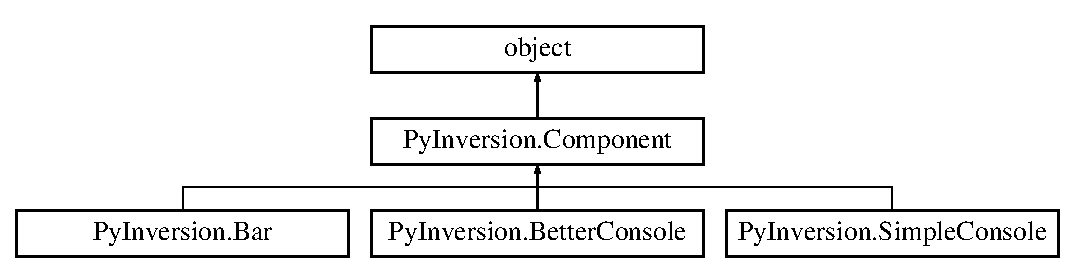
\includegraphics[height=3.000000cm]{class_py_inversion_1_1_component}
\end{center}
\end{figure}


The documentation for this class was generated from the following file\+:\begin{DoxyCompactItemize}
\item 
D\+:/\+Dropbox/\+A\+S\+C\+O\+N\+Projects/\+Py\+Patterns/\hyperlink{_py_inversion_8py}{Py\+Inversion.\+py}\end{DoxyCompactItemize}

\hypertarget{class_py_inversion_1_1_feature_broker}{\section{Py\+Inversion.\+Feature\+Broker Class Reference}
\label{class_py_inversion_1_1_feature_broker}\index{Py\+Inversion.\+Feature\+Broker@{Py\+Inversion.\+Feature\+Broker}}
}


Feature Broker.  


\subsection*{Public Member Functions}
\begin{DoxyCompactItemize}
\item 
def \hyperlink{class_py_inversion_1_1_feature_broker_a175067675b251079ca1d80e4aed4864d}{\+\_\+\+\_\+init\+\_\+\+\_\+}
\item 
def \hyperlink{class_py_inversion_1_1_feature_broker_ab9530aada9d12386127d047cd1307aa0}{Provide}
\item 
def \hyperlink{class_py_inversion_1_1_feature_broker_a064332733ed0f5f7826a924f7ebb0684}{\+\_\+\+\_\+getitem\+\_\+\+\_\+}
\end{DoxyCompactItemize}
\subsection*{Public Attributes}
\begin{DoxyCompactItemize}
\item 
\hyperlink{class_py_inversion_1_1_feature_broker_ab400ab32713a1a15bbf13f1cd901d9eb}{providers}
\item 
\hyperlink{class_py_inversion_1_1_feature_broker_a563bc54029c34054f768844c440aa5eb}{allow\+Replace}
\end{DoxyCompactItemize}


\subsection{Detailed Description}
Feature Broker. 



\subsection{Constructor \& Destructor Documentation}
\hypertarget{class_py_inversion_1_1_feature_broker_a175067675b251079ca1d80e4aed4864d}{\index{Py\+Inversion\+::\+Feature\+Broker@{Py\+Inversion\+::\+Feature\+Broker}!\+\_\+\+\_\+init\+\_\+\+\_\+@{\+\_\+\+\_\+init\+\_\+\+\_\+}}
\index{\+\_\+\+\_\+init\+\_\+\+\_\+@{\+\_\+\+\_\+init\+\_\+\+\_\+}!Py\+Inversion\+::\+Feature\+Broker@{Py\+Inversion\+::\+Feature\+Broker}}
\subsubsection[{\+\_\+\+\_\+init\+\_\+\+\_\+}]{\setlength{\rightskip}{0pt plus 5cm}def Py\+Inversion.\+Feature\+Broker.\+\_\+\+\_\+init\+\_\+\+\_\+ (
\begin{DoxyParamCaption}
\item[{}]{self, }
\item[{}]{allow\+Replace = {\ttfamily False}}
\end{DoxyParamCaption}
)}}\label{class_py_inversion_1_1_feature_broker_a175067675b251079ca1d80e4aed4864d}


\subsection{Member Function Documentation}
\hypertarget{class_py_inversion_1_1_feature_broker_a064332733ed0f5f7826a924f7ebb0684}{\index{Py\+Inversion\+::\+Feature\+Broker@{Py\+Inversion\+::\+Feature\+Broker}!\+\_\+\+\_\+getitem\+\_\+\+\_\+@{\+\_\+\+\_\+getitem\+\_\+\+\_\+}}
\index{\+\_\+\+\_\+getitem\+\_\+\+\_\+@{\+\_\+\+\_\+getitem\+\_\+\+\_\+}!Py\+Inversion\+::\+Feature\+Broker@{Py\+Inversion\+::\+Feature\+Broker}}
\subsubsection[{\+\_\+\+\_\+getitem\+\_\+\+\_\+}]{\setlength{\rightskip}{0pt plus 5cm}def Py\+Inversion.\+Feature\+Broker.\+\_\+\+\_\+getitem\+\_\+\+\_\+ (
\begin{DoxyParamCaption}
\item[{}]{self, }
\item[{}]{feature}
\end{DoxyParamCaption}
)}}\label{class_py_inversion_1_1_feature_broker_a064332733ed0f5f7826a924f7ebb0684}
\hypertarget{class_py_inversion_1_1_feature_broker_ab9530aada9d12386127d047cd1307aa0}{\index{Py\+Inversion\+::\+Feature\+Broker@{Py\+Inversion\+::\+Feature\+Broker}!Provide@{Provide}}
\index{Provide@{Provide}!Py\+Inversion\+::\+Feature\+Broker@{Py\+Inversion\+::\+Feature\+Broker}}
\subsubsection[{Provide}]{\setlength{\rightskip}{0pt plus 5cm}def Py\+Inversion.\+Feature\+Broker.\+Provide (
\begin{DoxyParamCaption}
\item[{}]{self, }
\item[{}]{feature, }
\item[{}]{provider, }
\item[{}]{args, }
\item[{}]{kwargs}
\end{DoxyParamCaption}
)}}\label{class_py_inversion_1_1_feature_broker_ab9530aada9d12386127d047cd1307aa0}


\subsection{Member Data Documentation}
\hypertarget{class_py_inversion_1_1_feature_broker_a563bc54029c34054f768844c440aa5eb}{\index{Py\+Inversion\+::\+Feature\+Broker@{Py\+Inversion\+::\+Feature\+Broker}!allow\+Replace@{allow\+Replace}}
\index{allow\+Replace@{allow\+Replace}!Py\+Inversion\+::\+Feature\+Broker@{Py\+Inversion\+::\+Feature\+Broker}}
\subsubsection[{allow\+Replace}]{\setlength{\rightskip}{0pt plus 5cm}Py\+Inversion.\+Feature\+Broker.\+allow\+Replace}}\label{class_py_inversion_1_1_feature_broker_a563bc54029c34054f768844c440aa5eb}
\hypertarget{class_py_inversion_1_1_feature_broker_ab400ab32713a1a15bbf13f1cd901d9eb}{\index{Py\+Inversion\+::\+Feature\+Broker@{Py\+Inversion\+::\+Feature\+Broker}!providers@{providers}}
\index{providers@{providers}!Py\+Inversion\+::\+Feature\+Broker@{Py\+Inversion\+::\+Feature\+Broker}}
\subsubsection[{providers}]{\setlength{\rightskip}{0pt plus 5cm}Py\+Inversion.\+Feature\+Broker.\+providers}}\label{class_py_inversion_1_1_feature_broker_ab400ab32713a1a15bbf13f1cd901d9eb}


The documentation for this class was generated from the following file\+:\begin{DoxyCompactItemize}
\item 
D\+:/\+Dropbox/\+A\+S\+C\+O\+N\+Projects/\+Py\+Patterns/\hyperlink{_py_inversion_8py}{Py\+Inversion.\+py}\end{DoxyCompactItemize}

\hypertarget{classzrpcserver_1_1_hello_r_p_c}{\section{zrpcserver.\+Hello\+R\+P\+C Class Reference}
\label{classzrpcserver_1_1_hello_r_p_c}\index{zrpcserver.\+Hello\+R\+P\+C@{zrpcserver.\+Hello\+R\+P\+C}}
}
Inheritance diagram for zrpcserver.\+Hello\+R\+P\+C\+:\begin{figure}[H]
\begin{center}
\leavevmode
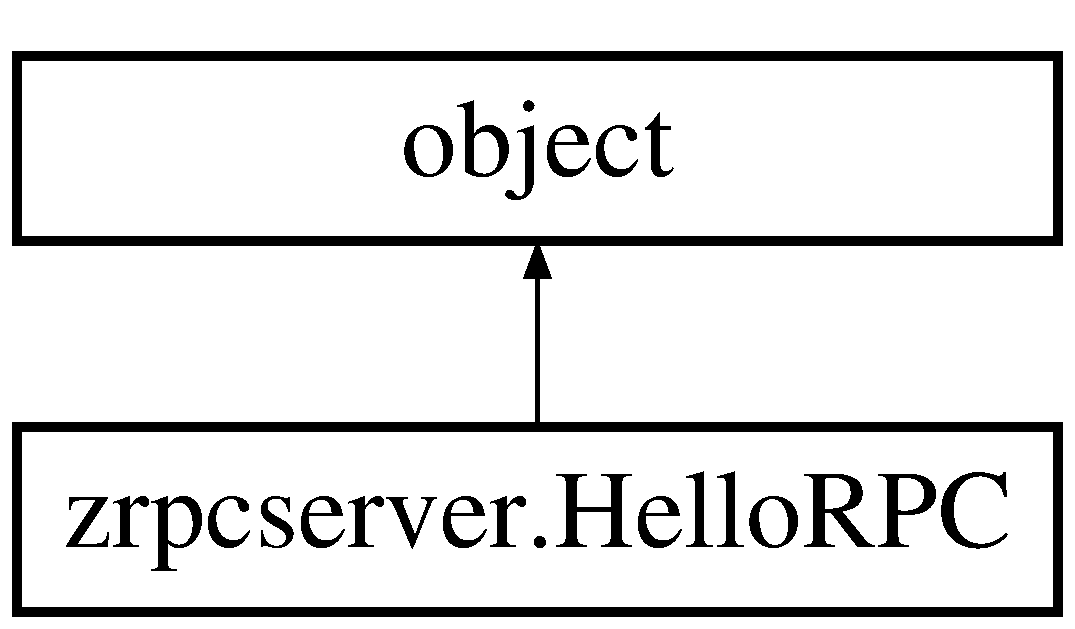
\includegraphics[height=2.000000cm]{classzrpcserver_1_1_hello_r_p_c}
\end{center}
\end{figure}
\subsection*{Public Member Functions}
\begin{DoxyCompactItemize}
\item 
def \hyperlink{classzrpcserver_1_1_hello_r_p_c_ac6dad4fb1eb5c1a2ce4261bf182eead0}{hello}
\end{DoxyCompactItemize}


\subsection{Member Function Documentation}
\hypertarget{classzrpcserver_1_1_hello_r_p_c_ac6dad4fb1eb5c1a2ce4261bf182eead0}{\index{zrpcserver\+::\+Hello\+R\+P\+C@{zrpcserver\+::\+Hello\+R\+P\+C}!hello@{hello}}
\index{hello@{hello}!zrpcserver\+::\+Hello\+R\+P\+C@{zrpcserver\+::\+Hello\+R\+P\+C}}
\subsubsection[{hello}]{\setlength{\rightskip}{0pt plus 5cm}def zrpcserver.\+Hello\+R\+P\+C.\+hello (
\begin{DoxyParamCaption}
\item[{}]{self, }
\item[{}]{name}
\end{DoxyParamCaption}
)}}\label{classzrpcserver_1_1_hello_r_p_c_ac6dad4fb1eb5c1a2ce4261bf182eead0}


The documentation for this class was generated from the following file\+:\begin{DoxyCompactItemize}
\item 
D\+:/\+Dropbox/\+A\+S\+C\+O\+N\+Projects/\+Py\+Patterns/\hyperlink{zrpcserver_8py}{zrpcserver.\+py}\end{DoxyCompactItemize}

\hypertarget{class_py_inversion_1_1_required_feature}{\section{Py\+Inversion.\+Required\+Feature Class Reference}
\label{class_py_inversion_1_1_required_feature}\index{Py\+Inversion.\+Required\+Feature@{Py\+Inversion.\+Required\+Feature}}
}
Inheritance diagram for Py\+Inversion.\+Required\+Feature\+:\begin{figure}[H]
\begin{center}
\leavevmode
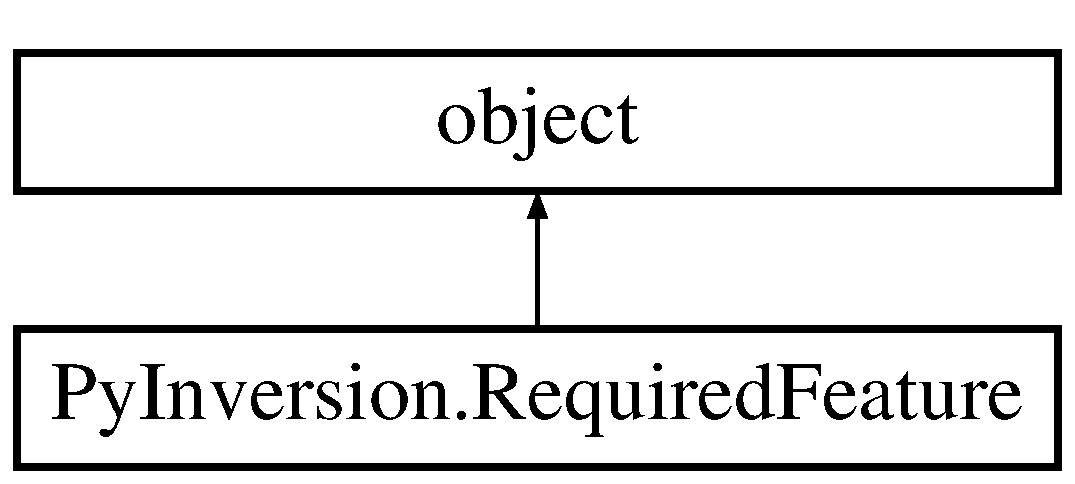
\includegraphics[height=2.000000cm]{class_py_inversion_1_1_required_feature}
\end{center}
\end{figure}
\subsection*{Public Member Functions}
\begin{DoxyCompactItemize}
\item 
def \hyperlink{class_py_inversion_1_1_required_feature_a375929df7e69c3007cca55f16734fea6}{\+\_\+\+\_\+init\+\_\+\+\_\+}
\item 
def \hyperlink{class_py_inversion_1_1_required_feature_a7d80a58ed26e163ce5378d4c85b30acf}{\+\_\+\+\_\+get\+\_\+\+\_\+}
\item 
def \hyperlink{class_py_inversion_1_1_required_feature_aa80602fe78081b4b4397ea2525b1f8ed}{\+\_\+\+\_\+getattr\+\_\+\+\_\+}
\item 
def \hyperlink{class_py_inversion_1_1_required_feature_a6b5ba6d11ef85d9295a567a441e8432a}{Request}
\end{DoxyCompactItemize}
\subsection*{Public Attributes}
\begin{DoxyCompactItemize}
\item 
\hyperlink{class_py_inversion_1_1_required_feature_a9d27890fe52489cae6ba6e692e856c33}{feature}
\item 
\hyperlink{class_py_inversion_1_1_required_feature_aa20d4e8ea16793c413631def7daf0caf}{assertion}
\item 
\hyperlink{class_py_inversion_1_1_required_feature_a3cc2960e714d44ebf6c440ff99aedbf5}{result}
\end{DoxyCompactItemize}


\subsection{Constructor \& Destructor Documentation}
\hypertarget{class_py_inversion_1_1_required_feature_a375929df7e69c3007cca55f16734fea6}{\index{Py\+Inversion\+::\+Required\+Feature@{Py\+Inversion\+::\+Required\+Feature}!\+\_\+\+\_\+init\+\_\+\+\_\+@{\+\_\+\+\_\+init\+\_\+\+\_\+}}
\index{\+\_\+\+\_\+init\+\_\+\+\_\+@{\+\_\+\+\_\+init\+\_\+\+\_\+}!Py\+Inversion\+::\+Required\+Feature@{Py\+Inversion\+::\+Required\+Feature}}
\subsubsection[{\+\_\+\+\_\+init\+\_\+\+\_\+}]{\setlength{\rightskip}{0pt plus 5cm}def Py\+Inversion.\+Required\+Feature.\+\_\+\+\_\+init\+\_\+\+\_\+ (
\begin{DoxyParamCaption}
\item[{}]{self, }
\item[{}]{feature, }
\item[{}]{assertion = {\ttfamily {\bf No\+Assertion}}}
\end{DoxyParamCaption}
)}}\label{class_py_inversion_1_1_required_feature_a375929df7e69c3007cca55f16734fea6}


\subsection{Member Function Documentation}
\hypertarget{class_py_inversion_1_1_required_feature_a7d80a58ed26e163ce5378d4c85b30acf}{\index{Py\+Inversion\+::\+Required\+Feature@{Py\+Inversion\+::\+Required\+Feature}!\+\_\+\+\_\+get\+\_\+\+\_\+@{\+\_\+\+\_\+get\+\_\+\+\_\+}}
\index{\+\_\+\+\_\+get\+\_\+\+\_\+@{\+\_\+\+\_\+get\+\_\+\+\_\+}!Py\+Inversion\+::\+Required\+Feature@{Py\+Inversion\+::\+Required\+Feature}}
\subsubsection[{\+\_\+\+\_\+get\+\_\+\+\_\+}]{\setlength{\rightskip}{0pt plus 5cm}def Py\+Inversion.\+Required\+Feature.\+\_\+\+\_\+get\+\_\+\+\_\+ (
\begin{DoxyParamCaption}
\item[{}]{self, }
\item[{}]{obj, }
\item[{}]{T}
\end{DoxyParamCaption}
)}}\label{class_py_inversion_1_1_required_feature_a7d80a58ed26e163ce5378d4c85b30acf}
\hypertarget{class_py_inversion_1_1_required_feature_aa80602fe78081b4b4397ea2525b1f8ed}{\index{Py\+Inversion\+::\+Required\+Feature@{Py\+Inversion\+::\+Required\+Feature}!\+\_\+\+\_\+getattr\+\_\+\+\_\+@{\+\_\+\+\_\+getattr\+\_\+\+\_\+}}
\index{\+\_\+\+\_\+getattr\+\_\+\+\_\+@{\+\_\+\+\_\+getattr\+\_\+\+\_\+}!Py\+Inversion\+::\+Required\+Feature@{Py\+Inversion\+::\+Required\+Feature}}
\subsubsection[{\+\_\+\+\_\+getattr\+\_\+\+\_\+}]{\setlength{\rightskip}{0pt plus 5cm}def Py\+Inversion.\+Required\+Feature.\+\_\+\+\_\+getattr\+\_\+\+\_\+ (
\begin{DoxyParamCaption}
\item[{}]{self, }
\item[{}]{name}
\end{DoxyParamCaption}
)}}\label{class_py_inversion_1_1_required_feature_aa80602fe78081b4b4397ea2525b1f8ed}
\hypertarget{class_py_inversion_1_1_required_feature_a6b5ba6d11ef85d9295a567a441e8432a}{\index{Py\+Inversion\+::\+Required\+Feature@{Py\+Inversion\+::\+Required\+Feature}!Request@{Request}}
\index{Request@{Request}!Py\+Inversion\+::\+Required\+Feature@{Py\+Inversion\+::\+Required\+Feature}}
\subsubsection[{Request}]{\setlength{\rightskip}{0pt plus 5cm}def Py\+Inversion.\+Required\+Feature.\+Request (
\begin{DoxyParamCaption}
\item[{}]{self}
\end{DoxyParamCaption}
)}}\label{class_py_inversion_1_1_required_feature_a6b5ba6d11ef85d9295a567a441e8432a}


\subsection{Member Data Documentation}
\hypertarget{class_py_inversion_1_1_required_feature_aa20d4e8ea16793c413631def7daf0caf}{\index{Py\+Inversion\+::\+Required\+Feature@{Py\+Inversion\+::\+Required\+Feature}!assertion@{assertion}}
\index{assertion@{assertion}!Py\+Inversion\+::\+Required\+Feature@{Py\+Inversion\+::\+Required\+Feature}}
\subsubsection[{assertion}]{\setlength{\rightskip}{0pt plus 5cm}Py\+Inversion.\+Required\+Feature.\+assertion}}\label{class_py_inversion_1_1_required_feature_aa20d4e8ea16793c413631def7daf0caf}
\hypertarget{class_py_inversion_1_1_required_feature_a9d27890fe52489cae6ba6e692e856c33}{\index{Py\+Inversion\+::\+Required\+Feature@{Py\+Inversion\+::\+Required\+Feature}!feature@{feature}}
\index{feature@{feature}!Py\+Inversion\+::\+Required\+Feature@{Py\+Inversion\+::\+Required\+Feature}}
\subsubsection[{feature}]{\setlength{\rightskip}{0pt plus 5cm}Py\+Inversion.\+Required\+Feature.\+feature}}\label{class_py_inversion_1_1_required_feature_a9d27890fe52489cae6ba6e692e856c33}
\hypertarget{class_py_inversion_1_1_required_feature_a3cc2960e714d44ebf6c440ff99aedbf5}{\index{Py\+Inversion\+::\+Required\+Feature@{Py\+Inversion\+::\+Required\+Feature}!result@{result}}
\index{result@{result}!Py\+Inversion\+::\+Required\+Feature@{Py\+Inversion\+::\+Required\+Feature}}
\subsubsection[{result}]{\setlength{\rightskip}{0pt plus 5cm}Py\+Inversion.\+Required\+Feature.\+result}}\label{class_py_inversion_1_1_required_feature_a3cc2960e714d44ebf6c440ff99aedbf5}


The documentation for this class was generated from the following file\+:\begin{DoxyCompactItemize}
\item 
D\+:/\+Dropbox/\+A\+S\+C\+O\+N\+Projects/\+Py\+Patterns/\hyperlink{_py_inversion_8py}{Py\+Inversion.\+py}\end{DoxyCompactItemize}

\hypertarget{class_py_inversion_1_1_simple_console}{\section{Py\+Inversion.\+Simple\+Console Class Reference}
\label{class_py_inversion_1_1_simple_console}\index{Py\+Inversion.\+Simple\+Console@{Py\+Inversion.\+Simple\+Console}}
}
Inheritance diagram for Py\+Inversion.\+Simple\+Console\+:\begin{figure}[H]
\begin{center}
\leavevmode
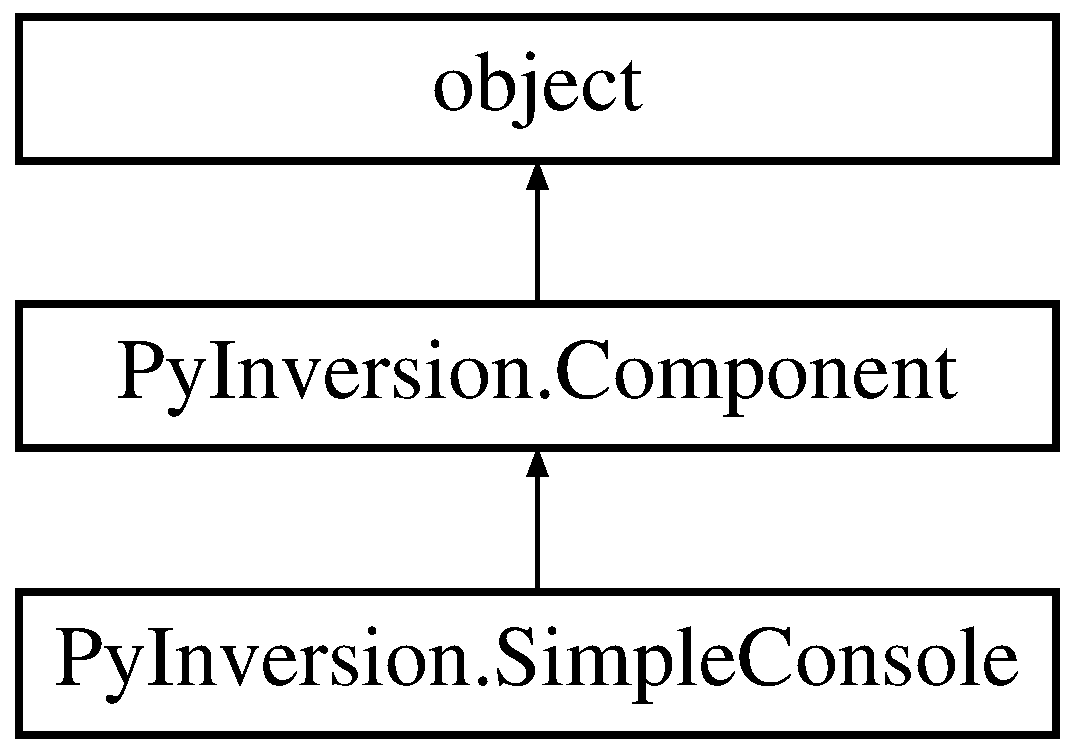
\includegraphics[height=3.000000cm]{class_py_inversion_1_1_simple_console}
\end{center}
\end{figure}
\subsection*{Public Member Functions}
\begin{DoxyCompactItemize}
\item 
def \hyperlink{class_py_inversion_1_1_simple_console_a394ab4167c1061bea32bd03a486d2862}{Write\+Line}
\end{DoxyCompactItemize}


\subsection{Member Function Documentation}
\hypertarget{class_py_inversion_1_1_simple_console_a394ab4167c1061bea32bd03a486d2862}{\index{Py\+Inversion\+::\+Simple\+Console@{Py\+Inversion\+::\+Simple\+Console}!Write\+Line@{Write\+Line}}
\index{Write\+Line@{Write\+Line}!Py\+Inversion\+::\+Simple\+Console@{Py\+Inversion\+::\+Simple\+Console}}
\subsubsection[{Write\+Line}]{\setlength{\rightskip}{0pt plus 5cm}def Py\+Inversion.\+Simple\+Console.\+Write\+Line (
\begin{DoxyParamCaption}
\item[{}]{self, }
\item[{}]{s}
\end{DoxyParamCaption}
)}}\label{class_py_inversion_1_1_simple_console_a394ab4167c1061bea32bd03a486d2862}


The documentation for this class was generated from the following file\+:\begin{DoxyCompactItemize}
\item 
D\+:/\+Dropbox/\+A\+S\+C\+O\+N\+Projects/\+Py\+Patterns/\hyperlink{_py_inversion_8py}{Py\+Inversion.\+py}\end{DoxyCompactItemize}

\chapter{File Documentation}
\hypertarget{categories_8py}{\section{D\+:/\+Dropbox/\+A\+S\+C\+O\+N\+Projects/\+Py\+Patterns/categories.py File Reference}
\label{categories_8py}\index{D\+:/\+Dropbox/\+A\+S\+C\+O\+N\+Projects/\+Py\+Patterns/categories.\+py@{D\+:/\+Dropbox/\+A\+S\+C\+O\+N\+Projects/\+Py\+Patterns/categories.\+py}}
}
\subsection*{Namespaces}
\begin{DoxyCompactItemize}
\item 
 \hyperlink{namespacecategories}{categories}
\end{DoxyCompactItemize}
\subsection*{Functions}
\begin{DoxyCompactItemize}
\item 
def \hyperlink{namespacecategories_ad5d3141fa655736c1fccef95069bf138}{categories.\+identity}
\item 
def \hyperlink{namespacecategories_a8c3eb907e91bca8102418150ca6db3fd}{categories.\+plusone}
\item 
def \hyperlink{namespacecategories_a4e763f6d2815828e12fcfea9bc54ddb8}{categories.\+comp}
\end{DoxyCompactItemize}
\subsection*{Variables}
\begin{DoxyCompactItemize}
\item 
tuple \hyperlink{namespacecategories_aa6ad1b25eda2dc4703279de8c42636c3}{categories.\+a} = identity(\char`\"{}11\char`\"{})
\end{DoxyCompactItemize}

\hypertarget{_py_inversion_8py}{\section{D\+:/\+Dropbox/\+A\+S\+C\+O\+N\+Projects/\+Py\+Patterns/\+Py\+Inversion.py File Reference}
\label{_py_inversion_8py}\index{D\+:/\+Dropbox/\+A\+S\+C\+O\+N\+Projects/\+Py\+Patterns/\+Py\+Inversion.\+py@{D\+:/\+Dropbox/\+A\+S\+C\+O\+N\+Projects/\+Py\+Patterns/\+Py\+Inversion.\+py}}
}
\subsection*{Classes}
\begin{DoxyCompactItemize}
\item 
class \hyperlink{class_py_inversion_1_1_feature_broker}{Py\+Inversion.\+Feature\+Broker}
\begin{DoxyCompactList}\small\item\em Feature Broker. \end{DoxyCompactList}\item 
class \hyperlink{class_py_inversion_1_1_required_feature}{Py\+Inversion.\+Required\+Feature}
\item 
class \hyperlink{class_py_inversion_1_1_component}{Py\+Inversion.\+Component}
\item 
class \hyperlink{class_py_inversion_1_1_bar}{Py\+Inversion.\+Bar}
\begin{DoxyCompactList}\small\item\em D\+E\+M\+O. \end{DoxyCompactList}\item 
class \hyperlink{class_py_inversion_1_1_simple_console}{Py\+Inversion.\+Simple\+Console}
\item 
class \hyperlink{class_py_inversion_1_1_better_console}{Py\+Inversion.\+Better\+Console}
\end{DoxyCompactItemize}
\subsection*{Namespaces}
\begin{DoxyCompactItemize}
\item 
 \hyperlink{namespace_py_inversion}{Py\+Inversion}
\end{DoxyCompactItemize}
\subsection*{Functions}
\begin{DoxyCompactItemize}
\item 
def \hyperlink{namespace_py_inversion_a188b1a2e50ba7079abd28f76308d8ee1}{Py\+Inversion.\+No\+Assertion}
\begin{DoxyCompactList}\small\item\em Representation of Required Features and Feature Assertions. \end{DoxyCompactList}\item 
def \hyperlink{namespace_py_inversion_aef868798a7eac8ca225dd912b28ee196}{Py\+Inversion.\+Is\+Instance\+Of}
\item 
def \hyperlink{namespace_py_inversion_ae61281915fdeaebe010d9660152ed2b5}{Py\+Inversion.\+Has\+Attributes}
\item 
def \hyperlink{namespace_py_inversion_aa26f41ad968118f6feb4f754492b9246}{Py\+Inversion.\+Has\+Methods}
\item 
def \hyperlink{namespace_py_inversion_aa73efe236b02a8a53f625fd15ec22ef2}{Py\+Inversion.\+Get\+Current\+User}
\end{DoxyCompactItemize}
\subsection*{Variables}
\begin{DoxyCompactItemize}
\item 
string \hyperlink{namespace_py_inversion_a75d60c831488f0073dfa93077eeb6645}{Py\+Inversion.\+\_\+\+\_\+author\+\_\+\+\_\+} = 'bausk'
\item 
tuple \hyperlink{namespace_py_inversion_a83916a9bd83dabb820f9756e0d6e9bc5}{Py\+Inversion.\+features} = Feature\+Broker()
\item 
tuple \hyperlink{namespace_py_inversion_a2744d30b0d1932d2fc87d21291bb5a1a}{Py\+Inversion.\+bar} = Bar()
\begin{DoxyCompactList}\small\item\em features.\+Provide('Console', \hyperlink{class_py_inversion_1_1_better_console}{Better\+Console}(prefix='--$>$')) \# $<$-- singleton lifestyle \end{DoxyCompactList}\end{DoxyCompactItemize}

\hypertarget{zrpc2_8py}{\section{D\+:/\+Dropbox/\+A\+S\+C\+O\+N\+Projects/\+Py\+Patterns/zrpc2.py File Reference}
\label{zrpc2_8py}\index{D\+:/\+Dropbox/\+A\+S\+C\+O\+N\+Projects/\+Py\+Patterns/zrpc2.\+py@{D\+:/\+Dropbox/\+A\+S\+C\+O\+N\+Projects/\+Py\+Patterns/zrpc2.\+py}}
}
\subsection*{Namespaces}
\begin{DoxyCompactItemize}
\item 
 \hyperlink{namespacezrpc2}{zrpc2}
\end{DoxyCompactItemize}
\subsection*{Variables}
\begin{DoxyCompactItemize}
\item 
string \hyperlink{namespacezrpc2_ab6eb50c4b8d874520e4089b273b63e16}{zrpc2.\+\_\+\+\_\+author\+\_\+\+\_\+} = 'bausk'
\item 
tuple \hyperlink{namespacezrpc2_aad77b0202c8bdc01b68d63c381d5bb4b}{zrpc2.\+context} = zmq.\+Context()
\item 
tuple \hyperlink{namespacezrpc2_a5cc44b717d0374316398080bedecec05}{zrpc2.\+socket} = context.\+socket(zmq.\+R\+E\+P)
\item 
tuple \hyperlink{namespacezrpc2_a3a2870282951b1ba168443ba71d13079}{zrpc2.\+message} = socket.\+recv()
\item 
tuple \hyperlink{namespacezrpc2_a55892ab0cec9d46ce8b2a50f92998e57}{zrpc2.\+m2} = msgpack.\+unpackb(message)
\end{DoxyCompactItemize}

\hypertarget{zrpcclient_8py}{\section{D\+:/\+Dropbox/\+A\+S\+C\+O\+N\+Projects/\+Py\+Patterns/zrpcclient.py File Reference}
\label{zrpcclient_8py}\index{D\+:/\+Dropbox/\+A\+S\+C\+O\+N\+Projects/\+Py\+Patterns/zrpcclient.\+py@{D\+:/\+Dropbox/\+A\+S\+C\+O\+N\+Projects/\+Py\+Patterns/zrpcclient.\+py}}
}
\subsection*{Namespaces}
\begin{DoxyCompactItemize}
\item 
 \hyperlink{namespacezrpcclient}{zrpcclient}
\end{DoxyCompactItemize}
\subsection*{Variables}
\begin{DoxyCompactItemize}
\item 
tuple \hyperlink{namespacezrpcclient_a039edf63871343a5809f1e216cc7e5cd}{zrpcclient.\+c} = zerorpc.\+Client()
\end{DoxyCompactItemize}

\hypertarget{zrpcserver_8py}{\section{D\+:/\+Dropbox/\+A\+S\+C\+O\+N\+Projects/\+Py\+Patterns/zrpcserver.py File Reference}
\label{zrpcserver_8py}\index{D\+:/\+Dropbox/\+A\+S\+C\+O\+N\+Projects/\+Py\+Patterns/zrpcserver.\+py@{D\+:/\+Dropbox/\+A\+S\+C\+O\+N\+Projects/\+Py\+Patterns/zrpcserver.\+py}}
}
\subsection*{Classes}
\begin{DoxyCompactItemize}
\item 
class \hyperlink{classzrpcserver_1_1_hello_r_p_c}{zrpcserver.\+Hello\+R\+P\+C}
\end{DoxyCompactItemize}
\subsection*{Namespaces}
\begin{DoxyCompactItemize}
\item 
 \hyperlink{namespacezrpcserver}{zrpcserver}
\end{DoxyCompactItemize}
\subsection*{Variables}
\begin{DoxyCompactItemize}
\item 
tuple \hyperlink{namespacezrpcserver_a27c4be0435b479044d8544312829e19f}{zrpcserver.\+s} = zerorpc.\+Server(Hello\+R\+P\+C())
\item 
tuple \hyperlink{namespacezrpcserver_aba2558901917b86cf74044e3313df8d8}{zrpcserver.\+context} = zmq.\+Context()
\item 
tuple \hyperlink{namespacezrpcserver_a5e4952d9f1e8548ca60fc87e02414711}{zrpcserver.\+socket} = context.\+socket(zmq.\+R\+E\+P)
\item 
tuple \hyperlink{namespacezrpcserver_a3cf2b2246b68a156037b2a86b71282ff}{zrpcserver.\+message} = socket.\+recv()
\item 
tuple \hyperlink{namespacezrpcserver_a867cc3b9e35ae551991976a86a47829d}{zrpcserver.\+m2} = msgpack.\+unpackb(message)
\end{DoxyCompactItemize}

%--- End generated contents ---

% Index
\newpage
\phantomsection
\addcontentsline{toc}{chapter}{Index}
\printindex

\end{document}
